\documentclass[a4paper]{article}

\usepackage[english]{babel}
\usepackage[utf8]{inputenc}
\usepackage{amsmath}
\usepackage{graphicx}
\usepackage[colorinlistoftodos]{todonotes}
\usepackage{float}
\usepackage{subcaption}
\usepackage{hyperref}
\usepackage[letterpaper,top=0.5cm,bottom=2cm,left=3cm,right=3cm,marginparwidth=1.75cm]{geometry}

\title{Introduction to Artificial Intelligence \\ Assignment 1}

\author{Anton Nekhaev BS21-07, \\ a.nekhaev@innopolis.university}

\date{Fall 2022}

\graphicspath{{Images/}}

\begin{document}
\maketitle

\section{Assumptions}
\begin{enumerate}
  \item Agent can not go out of bounds of field.
  \item Cost of horizontal, vertical and diagonal moving is 1 point. 
  \item When we randomly generate the map an agent spawns in $(0, 0)$ coordinate.
\end{enumerate}

\section{PEAS of Jack Sparrow}
\begin{enumerate}
    \item[] Performance measure - achieving the Dead Man’s Chest with a shortest existed path. 
    \item[] Environment - matrix $9 \times 9$
    \item[] Actuators - changing position on map, visiting Tortuga, killing Kraken
    \item[] Sensors - spyglass (depends on scenario), compass
\end{enumerate}

\section{Properties of the enviroment}
\begin{enumerate}
    \item[] Partially Observable - Jack Sparrow can see only in his perception zone.
    \item[] Single Agent - only agent can move on the map, other entities are static.
    \item[] Sequential - the current decision has consequences on future actions, so, if Jack has killed the Kraken he can move in Kraken's coordinates without damage.
    \item[] Dynamic - agent can change the enviroment by killing Kraken.
    \item[] Discrete - Jack Sparrow makes discreate steps from cell to cell.
    \item[] Known - our agent has a compass, so he knows where Dead Man's Chest and Tortuga Island are located.
\end{enumerate}

\section{Search algorithms}
\subsection{Backtracking search}
Backtracking search tries all paths and finds for shortest one. For the implementation I use recursive approach. Also I have a two dimensional array - \emph{map} with capacity $9 \times 9$, cell with index $(x,y)$ corresponds to the minimal length of path that needed to get to this coordinate. So, thanks to presence of map array we can make a optimization of algorithm: if on one step current path to $(x, y)$ coordinate is greater than value of \emph{map}$[x][y]$ then we can exit from this recursion leaf because every other path in this recursion branch will be greater that path that we have obtain on previous steps. Recursion ends when can not make move to another cell or speaking in another words: we can not make solution for adjacent cells better than already exists.
\subsection{A*}
A* wants to reach the target cell (if possible) from the starting cell as quickly as possible, comparing to Backtracking search A* does not tries all paths. To do that it, he goes to cell with the minimum value of \emph{$f$}, \emph{$f$} = \emph{$g$} + \emph{$h$}, where \emph{$g$} - amount of steps from initial start position and \emph{$h$} - heuristic value, the minimum number of steps you need to take to be on the Dead Men's Chest Island if you go regardless of opponents. So, for the implementation I use a priority queue, node of which can be compared according to \emph{$f$} and if \emph{$f$} values are equal, nodes will compare according to \emph{$h$} values. So, on each step we will pick the node with the least cost, try to go to adjecent cells if cost to them that we obtained on previous steps is greater then current cost. For the first time when we reach the Dead Men's Chest Island this path will be the answer. Also for optimization I use the same approach as in Backtrack search (read above).

% \subsection{Observations about algorithms and scenarios}
% There is no difference in algorithms implementation for 2 different scenarios, since Jack Sparrow can move one step per turn and can move horizontally, vertically and diagonally and regardless of the scenario, we must go through all the cells in our path, no matter how close they are to the enemy cells. In the case of Backtracking go to these cells, and in the case of A* add them to the priority queue. Thus, both the program execution and the run time for both scenarios will be the same (The run time will vary by a very small amount, which can be called an error due to the different CPU loads of the computer, just as the garbage collector can affect the run time). 

\section{Solution of the problem}
For solving the specific board I consider to ways of reaching the Dead's Men Chest:
\begin{enumerate}
    \item Direct way to Dead's Men Chest Island.
    \item Way to Dead's Men Chest Island through Tortuga island to ensure that Jack have ability to kill the Kraken on his way from Tortuga to Dead's Men Chest Island.
\end{enumerate}

\section{Maps}
In this section I propose to consider some notable maps.
\subsection*{Map legend:}
\begin{enumerate}
    \item [] J -- Jack Sparrow
    \item [] T -- Tortuga
    \item [] C -- Dead's Men Chest
    \item [] K -- Kraken
    \item [] R -- Rock
    \item [] DJ -- Davy Jones
    \item [] * \ \  -- Path
\end{enumerate}
\subsection{Interesting map}
In this subsection there is an interesting map. We need to go to Dead's Men Chest Island through Toruga Island.
\begin{figure}[H]
    \centering
    \subcaptionbox{Remarkable map A}{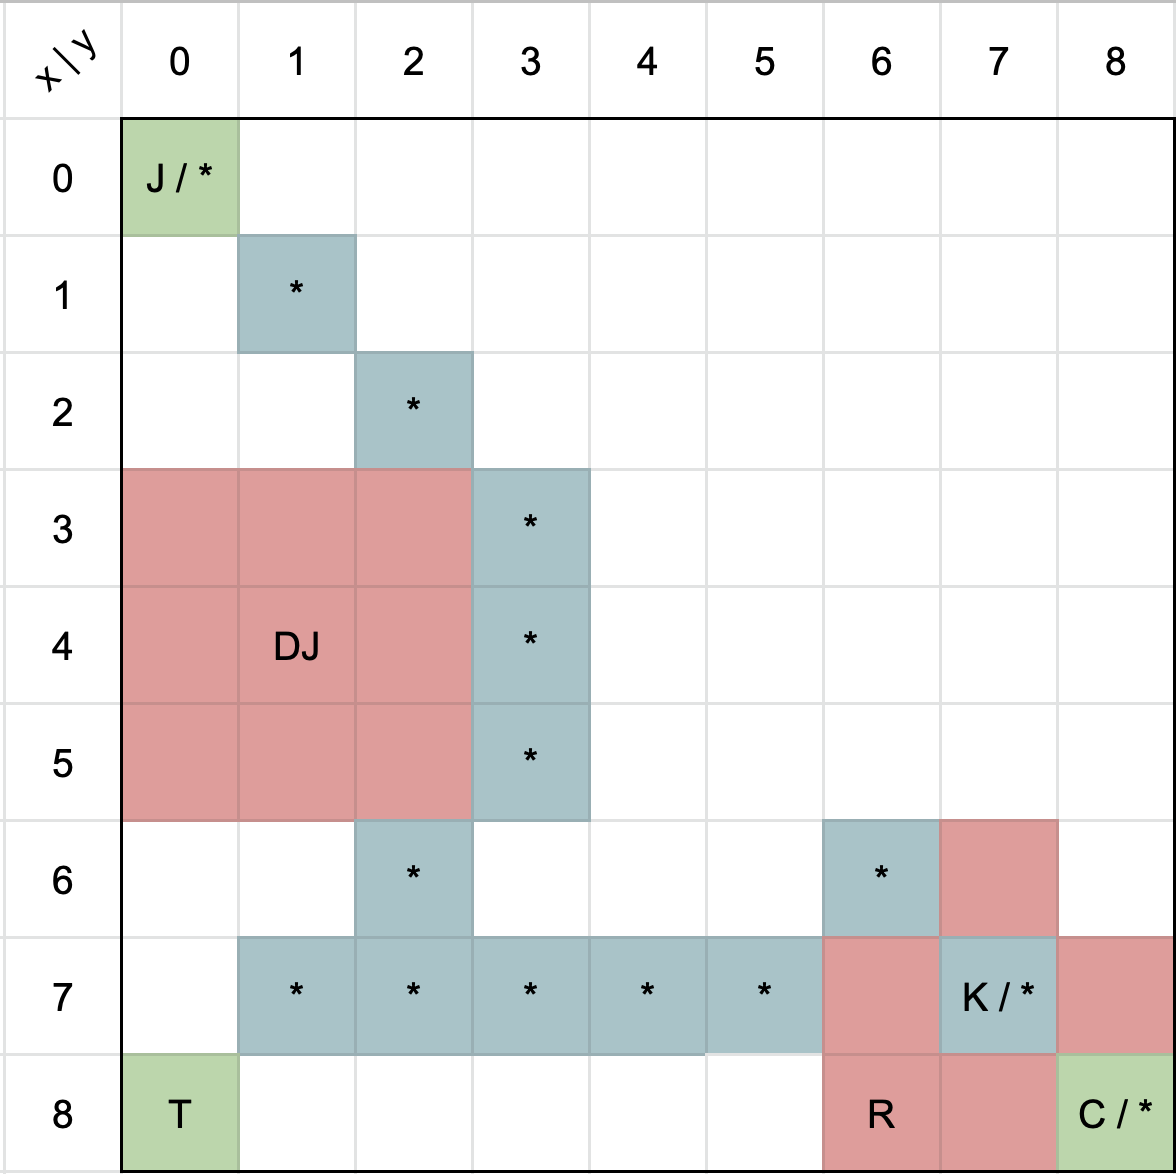
\includegraphics[width=0.5\textwidth]{Remarkable_map.png}}
\end{figure}

\subsection{Maps impossible to solve}
In this subsection there are maps (without their variations) that can not be solved using both algorithms, because on each map path to Dead's Men Chest does not exist.

\begin{figure}[H]
    \centering
    \subcaptionbox{Impossible map A}{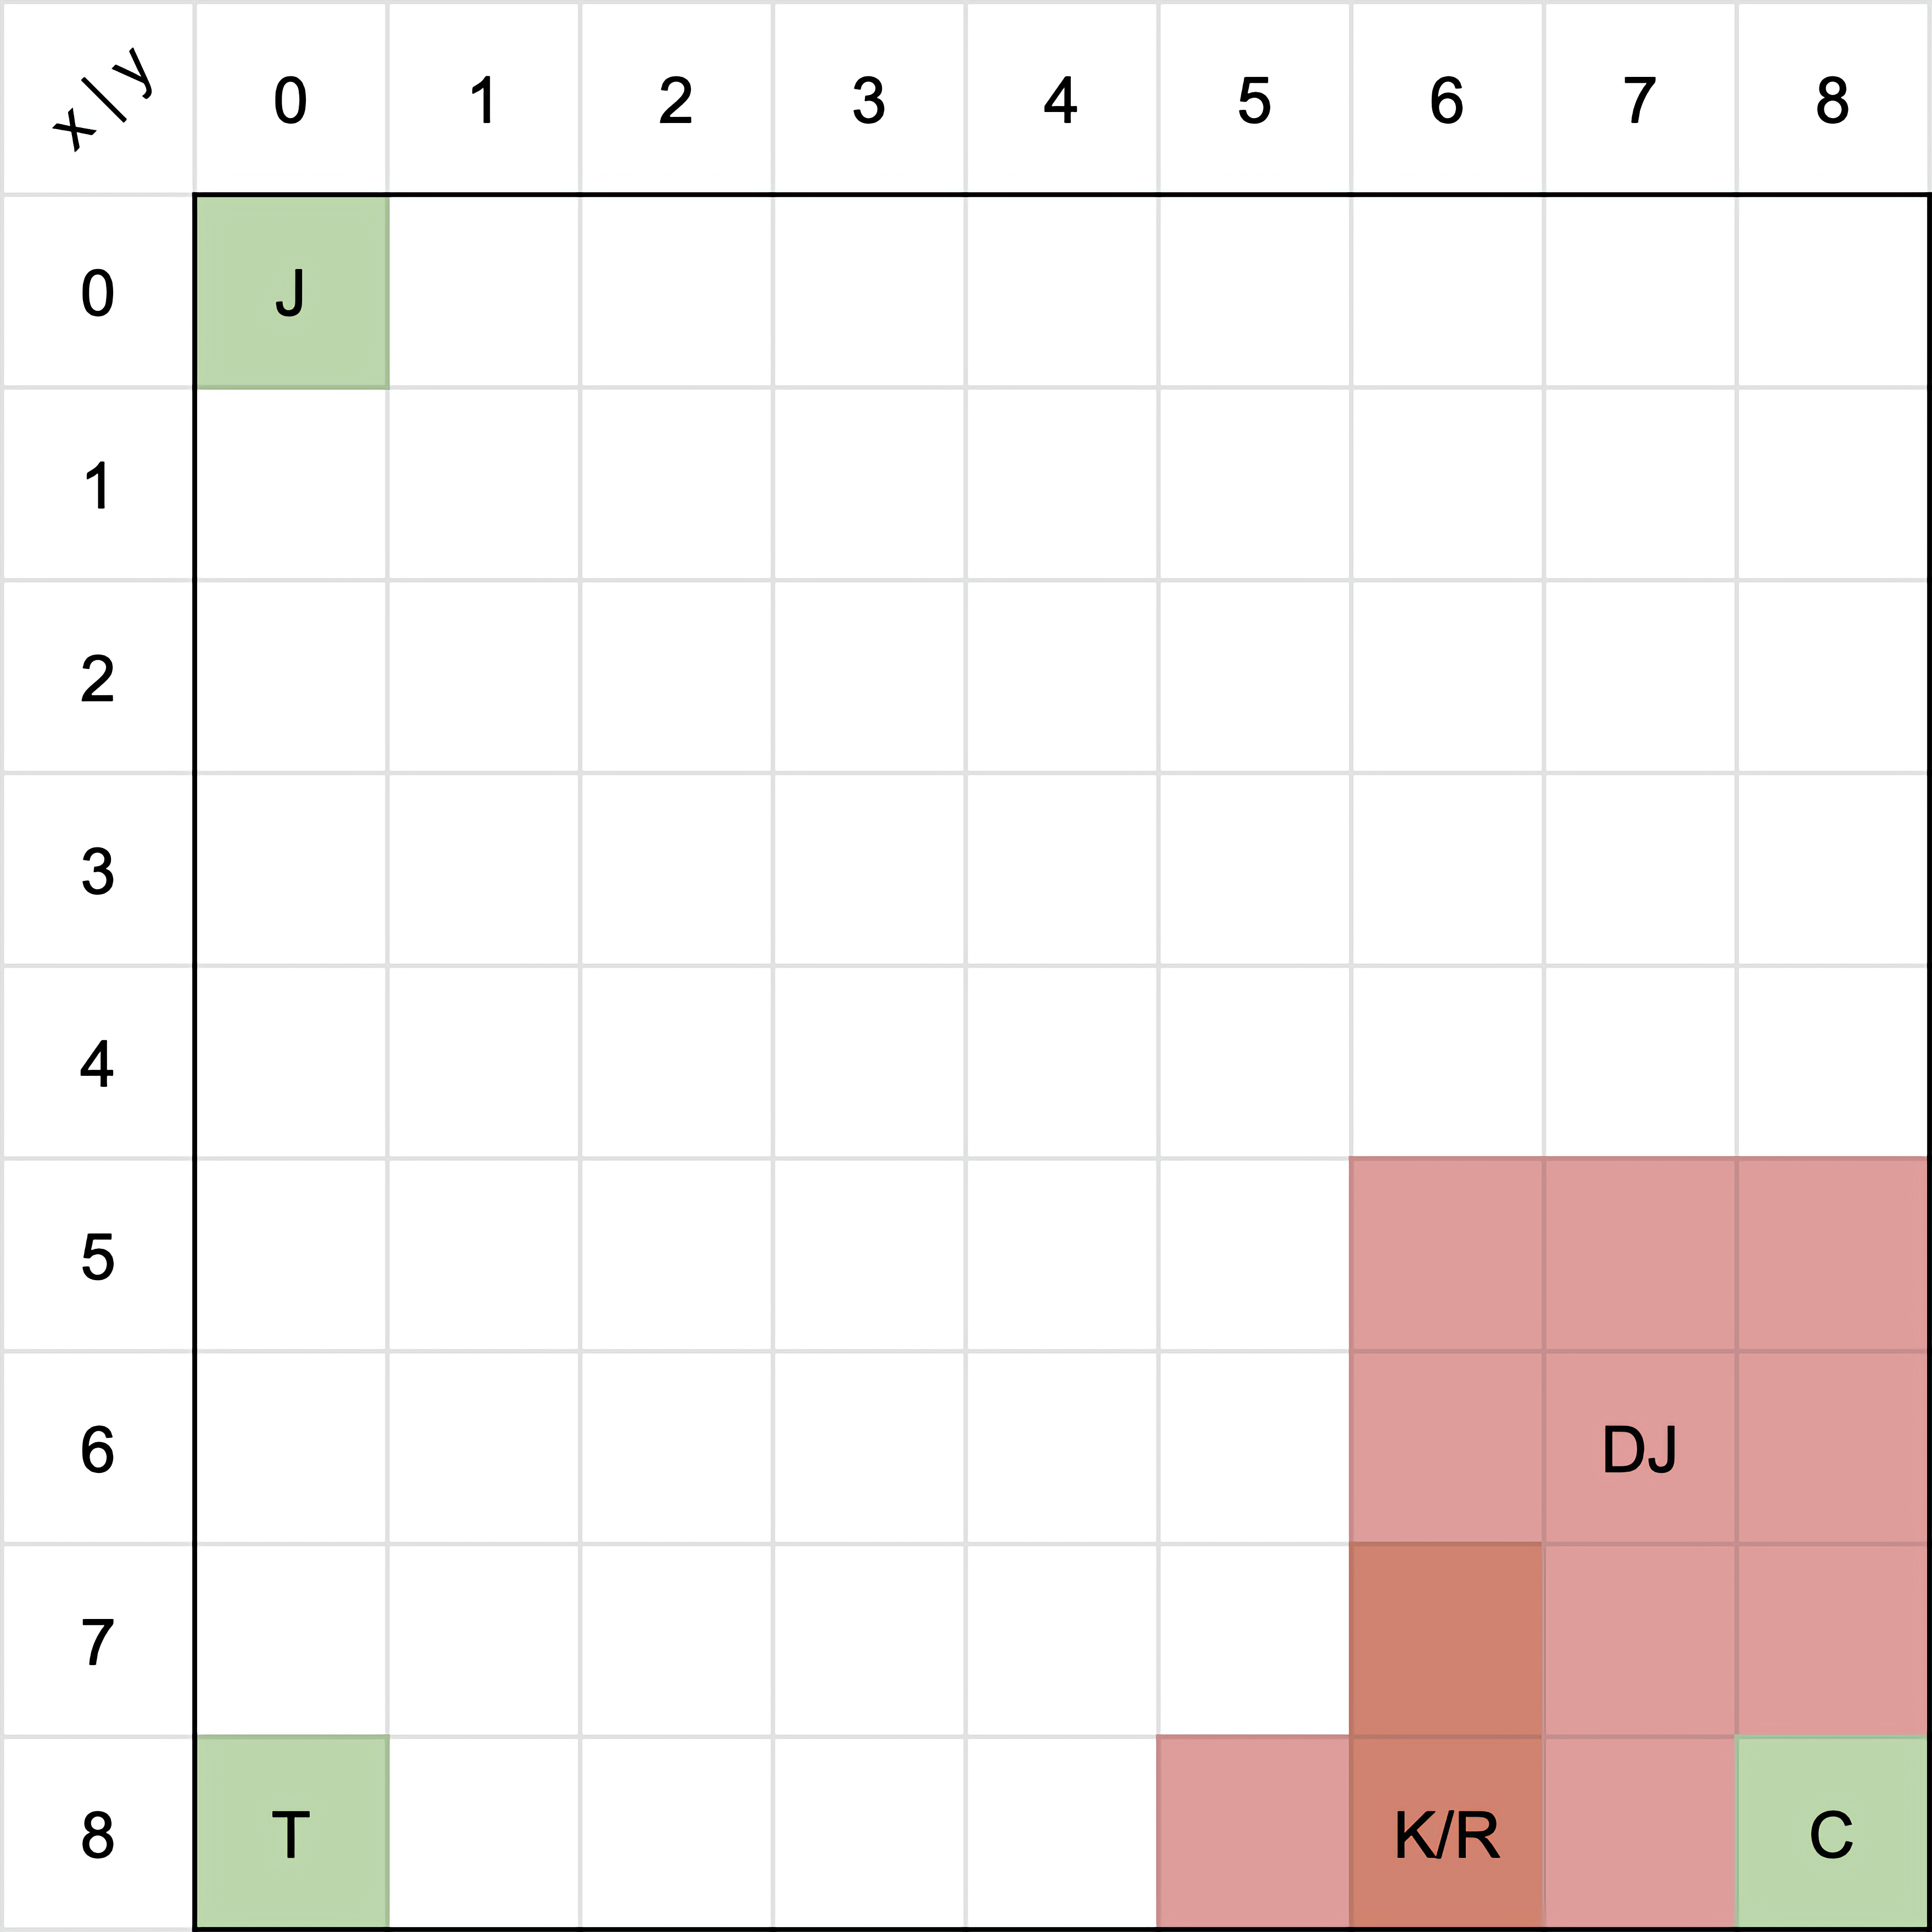
\includegraphics[width=0.33\textwidth]{impossible1.png}}
    \hfill % <-- Seperation
    \subcaptionbox{Impossible map B}{\includegraphics[width=0.33\textwidth]{impossible2.png}}
    \hfill
    \subcaptionbox{Impossible map C}{\includegraphics[width=0.33\textwidth]{impossible3.png}}
    \hfill
    \subcaptionbox{Impossible map D}{\includegraphics[width=0.33\textwidth]{impossible4.png}}
    \hfill
\end{figure}
\begin{enumerate}
    \item [(a)] -- Even if we kill the Kraken the path will be crossed by the stone.
    \item [(b)] -- It is impossible to visit the Tortuga to kill the Kraken afterwards.
    \item [(c)] -- Stone prevents the kraken from being killed.
    \item [(d)] -- Instance death for Jack Sparrow.
\end{enumerate}
\section{Statistical Analysis}
The analysis is based on 1000 runs of program, each program executes algoritms in 2 scenarios, that generate random map, each of which satisfies the task conditions. Let's compare!
\subsection*{Backtracking compared to A*} 

\begin{center}
\begin{tabular}{ |p{5cm}|p{2cm}|p{2cm}|p{2cm}|p{2cm}| }
    \hline
    & Backtracking&A*&Backtracking&A*\\
    \hline
    Scenario number&\multicolumn{2}{|c|}{1} & \multicolumn{2}{|c|}{2}\\
    \hline
    Mean of time for execution (ms)& 3.647 & 0.694 &2.627& 0.306\\
    Mode of time for execution (ms) & 3.62  & 0.63&2.64& 0.29\\
    Median of time for execution (ms)& 3.629 & 0.677&2.666& 0.296\\
    Standard deviation of time for execution (ms) & 3.662 & 0.712&2.674& 0.329\\
    \hline
    Number of wins & \multicolumn{4}{|c|}{942} \\
    Number of loses & \multicolumn{4}{|c|}{58}  \\
    Percentage of wins & \multicolumn{4}{|c|}{94.2\%} \\
    Percentage of loses & \multicolumn{4}{|c|}{5.8\%} \\
    \hline
\end{tabular}
\end{center}
As we see from the table A* solves this problem in less time than Backtracking in both scenarios, but algorithms show themselves the same when finding a path (if one algorithm finds a path, the second will find it too).\\
Also notable, if you compare the speed of the algorithm under different scenarios, you can see that the second scenario works faster than the first.

\section{Source code}
Java source code, together with files and python script for statistics are available on my Github repository, the \href{https://github.com/NAD777/AI-assignment-1}{link} (just click on it).
\end{document}